\section{Auswertung}
Für die Auswertung der Messdaten werden einige Fehlerrechnungen benötigt. Diese sind im Folgenden angegeben.
Alle Mittelwerte werden durch
\begin{equation}
    \label{eqn:mittel}
\bar{x} = \frac{1}{N} \sum_{i=1}^{N} x_{i}
\end{equation}
bestimmt, wobei $N$ die Anzahl der betrachten Messwerte angibt. Die Standardabweichung $\sigma$ einer Messreihe lässt sich folgendermaßen berechnen.
\begin{equation}
\sigma = \sqrt{\frac{1}{N-1}\sum_{i=1}^{N} (x_{i} -\bar{x})^2 }
\end{equation}
Der sogenannte Standardfehler des Mittelwerts ist durch eine Beziehung zur Standardabweichung definiert.
\begin{equation}
    \label{eqn:sem}
\increment \bar{x} = \frac{\sigma}{\sqrt{N}} = \frac{1}{\sqrt{N}} \sqrt{\frac{1}{N-1}\sum_{i=1}^{N} (x_{i} -\bar{x})^2 }
\end{equation}
Wenn Werte in einer beliebigen Berechnungsformel fehlerbehaftet sind kann der Fehler anhand der Gaußschen Fehlerfortpflanzung ermittelt werden. Diese sieht im allgemeinen Fall folgendermaßen aus.
\begin{equation}
    \label{eqn:gauss}
\increment f = \sqrt{\sum_{i=1}^{N} \left( \frac{\partial f}{\partial x_{i}}\right)^2 (\increment x_{i})^2}
\end{equation}
Es wird also über alle Variablen summiert welche einen Fehler $\increment x_{i}$ besitzen. Für Formeln mit nur einem fehlerbehafteten Wert vereinfacht sich die Gleichung dementsprechend.

\subsection{Statische Methode}
Zunächst lassen sich die Temperaturen ferner vom Pertier-Element graphisch darstellen. Dazu gehören also $T_{1}$, $T_{4}$, $T_{5}$ und $T_{8}$ also alle Temperaturen am Ende der einzelnen Metallstäbe.
Gemessen wurde über eine Dauer von $t = \SI{710}{\second}$ und die Temperatur $T_{7}$ erreicht niemals den Wert $\SI{45}{\celsius}$ also kann für diese Betrachtung das ganze Intervall verwendet werden.
Abbildung \ref{fig:plot1} zeigt die Temperaturen $T_{1}$ und $T_{4}$ also die unterschiedlichen Messingstäbe und Abbildung \ref{fig:plot2} die Temperaturen $T_{5}$ und $T_{8}$ also Aluminium und Edelstahl.

\begin{figure}
    \centering
    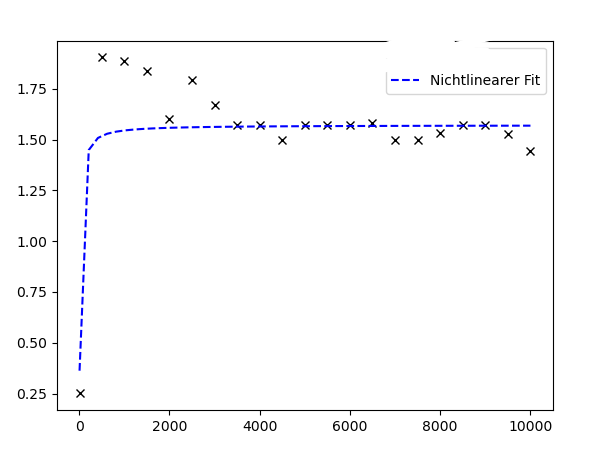
\includegraphics[width=\textwidth]{build/plot1.pdf}
    \caption{Temperaturverlauf der Messsonden T1 und T4 angebracht auf Messing} 
    \label{fig:plot1}
\end{figure}

\begin{figure}
    \centering
    \includegraphics[width=\textwidth]{build/plot2.pdf}
    \caption{Temperaturverlauf der Messsonden T5 (Aluminium) und T8(Edelstahl)} 
    \label{fig:plot2}
\end{figure}
\newpage
Erkennbar ist, dass alle Temperaturen einen annähernd logarithmischen Verlauf zeigen. 
Die beiden Messingstäbe in Abbildung \ref{fig:plot1} sind dabei zu Beginn identisch und unterscheiden sich erst ab einer Temperatur von $T = \SI{30}{\celsius}$, wobei der breitere Messingstab stärker wächst als der dünnere. Dies ist ebenfalls zu erwarten, da die Gleichung
\ref{eqn:itsHeadacheTimeYeeeay} proportional zum Querschnitt ist. Im groben Verlauf sind die beiden jedoch durch die gleiche Wärmeleitfähigkeit $\kappa_{\text{messing}}$ sehr ähnlich.
\\
Für die beiden Temperaturen $T_{5}$ und $T_{8}$ in Abbildung \ref{fig:plot2} sind größere Unterschiede zu erkennen. Die Temperatur im Edelstahl wächst nahezu linear und lässt somit auf eine eher kleine Wärmeleitfähigkeit schließen. Der 
Temperaturverlauf für Aluminium hingegen ist denen von Messing sehr ähnlich besitz allerdings eine noch größere Maximaltemperatur zum Schluss der Messung. 
\\
Die maximalen Temperaturen zum Zeitpunkt $t = \SI{710}{\second}$ sind im folgenden angegeben.
\begin{align}
    T_1 &= \SI{45.65}{\celsius} \\
    T_4 &= \SI{43.21}{\celsius} \\
    T_5 &= \SI{48.28}{\celsius} \\
    T_8 &= \SI{34.75}{\celsius}
\end{align}
Somit kann festgestellt werden, dass die Wärmeleitfähigkeit vom Aluminium $\kappa_{\text{alu}}$ am besten, also am größten ist.
\\
\newline
Mit den Literaturwerten für die Wärmeleitfähigkeit $\kappa$ kann nun zu verschiedenen Messzeiten der Wärmestrom $\increment Q$/$\increment t$ bestimmt werden. Dazu werden Messzeiten im Abstand von $\increment t = \SI{140}{\second}$
gewählt. Für die Bestimmung mit Gleichung \ref{eqn:itsHeadacheTimeYeeeay} wird ebenfalls die Querschnittsfläche der Stäbe benötigt. Diese unterscheidet sich nur bei dem einen schmalen Messingstab zu den drei sonst gleich großen Stäben.
Sie lassen sich mit den Werten aus Tabelle \ref{tab:einfach} berechnen. 
\begin{align}
A_{\text{breit}} &= \SI{48e-6}{\meter\squared}\\
A_{\text{schmal}} &= \SI{28e-6}{\meter\squared}
\end{align}
Zusammen mit dem Abstand zwischen den Thermoelementen $\increment x = \SI{0.03}{\meter}$ lassen sich diese Werte nun in Gleichung \ref{eqn:itsHeadacheTimeYeeeay} einsetzen. Die Tabellen \ref{tab:mesbreit} bis \ref{tab:edel} zeigen den bestimmten Wärmefluss
der einzelnen Stäbe.
\begin{table}
    \centering
    \caption{Wärmestrom vom breiten Messingstab.}
    \label{tab:mesbreit}
    \begin{tabular}{c c c}
        \toprule
        Messzeit $t$ [$\si{\second}$]   & $T_{2} - T_{1}$ [$\si{\kelvin}$] &  $\frac{\increment Q_{2 \to 1}}{\increment t}$ [$\si{\watt}$]  \\
        \midrule
        140     &   4.08   & -0.74   \\
        280     &   2.80   &  -0.51  \\
        420     &   2.42   &  -0.44  \\
        560     &   2.25   &   -0.41 \\
        700     &   2.21   &  -0.40  \\
        \bottomrule
    \end{tabular}
\end{table}
\begin{table}
    \centering
    \caption{Wärmestrom vom schmalen Messingstab.}
    \label{tab:messchmal}
    \begin{tabular}{c c c}
        \toprule
        Messzeit $t$ [$\si{\second}$]   & $T_{3} - T_{4}$ [$\si{\kelvin}$] &  $\frac{\increment Q_{3 \to 4}}{\increment t}$ [$\si{\watt}$]  \\
        \midrule
        140     &   4.99   & -0.53   \\
        280     &   3.86   &  -0.41  \\
        420     &   3.67   &  -0.39  \\
        560     &   3.63   &   -0.38 \\
        700     &   3.63   &  -0.38 \\
        \bottomrule
    \end{tabular}
\end{table}
\begin{table}
    \centering
    \caption{Wärmestrom vom Aluminiumstab.}
    \label{tab:alu}
    \begin{tabular}{c c c}
        \toprule
        Messzeit $t$ [$\si{\second}$]   & $T_{6} - T_{5}$ [$\si{\kelvin}$] &  $\frac{\increment Q_{6 \to 5}}{\increment t}$ [$\si{\watt}$]  \\
        \midrule
        140     &   2.59   & -0.91  \\
        280     &   1.72   &  -0.61  \\
        420     &   1.56   &  -0.55  \\
        560     &   1.51   &   -0.53 \\
        700     &   1.51   &  -0.53 \\
        \bottomrule
    \end{tabular}
\end{table}
\begin{table}
    \centering
    \caption{Wärmestrom vom Edelstahlstab.}
    \label{tab:edel}
    \begin{tabular}{c c c}
        \toprule
        Messzeit $t$ [$\si{\second}$]   & $T_{7} - T_{8}$ [$\si{\kelvin}$] &  $\frac{\increment Q_{7 \to 8}}{\increment t}$ [$\si{\watt}$]  \\
        \midrule
        140     &   9.16   & -0.31  \\
        280     &   9.55   &  -0.32  \\
        420     &   9.55   &  -0.32  \\
        560     &   9.54   &   -0.32 \\
        700     &   9.52   &  -0.32\\
        \bottomrule
    \end{tabular}
\end{table}

Zusätzlich lassen sich die Temperaturdifferenzen zwischen den beiden Enden eines Stabes graphisch darstellen. Im Folgenden wird die Differenz der gemessenen Werte $T_{7} - T_{8}$ und $T_{2} - T_{1}$, also des breiten Messing- und
Edelstahlstabs betrachtet. Dies ist in Abbildung \ref{fig:plot3} gezeigt.

\begin{figure}
    \centering
    \includegraphics[width=\textwidth]{build/plot3.pdf}
    \caption{Temperaturdifferenzen des Edelstahlstabs ($T_{7}-T_{8}$) und breiten Messingstabes ($T_{2}-T_{1}$).} 
    \label{fig:plot3}
\end{figure}

Deutlich zu erkennen ist die unterschiedliche Maximaltemperaturdifferenz der beiden Kurven. Beide verlaufen ab einem Punkt asymptotisch gegen einen Grenzwert. Für die Edelstahlkurve liegt der bei knapp $\SI{9.54}{\celsius}$ und bei der 
Messingkurve bei $\SI{2.21}{\celsius}$. Dies lässt auf deutlich zu erkennende Größenunterschiede in den Wärmeleitfähigkeiten $\kappa$ schließen, wobei $\kappa_{\text{edel}} < \kappa_{\text{messing}}$. Beide Kurven steigen zu
Beginn schnell an und mit der Zeit wird die Wärme von einem zum anderen Ende transportiert. Das Temperaturmaximum wird bei dem Edehlstahlstab ebenfalls früher erreicht.

\subsection{Dynamische Methode}
Mit dieser Methode können die Wärmeleitfähigkeiten $\kappa$ der einzelnen Metallstäbe bestimmt werden, dazu wurden die Stäbe periodisch aufgeheizt und abgekühlt mit einer Periodendauer von $T = \SI{200}{\second}$.
Zunächst wird hier der breite Messingstab betrachtet, dabei sind die Temperaturen $T_{1}$ und $T_{2}$ in der Abbildung \ref{fig:plot4} dargestellt. Aus dieser Graphik lassen sich die charakteristischen Eigenschaften der Temperaturwelle
ablesen. Dazu gehören die Amplituden der Temperaturen $A_{1}$ und $A_{2}$ sowie die Phasendifferenz $\increment t$.
Die ausgelesenen Werte sind in Tabelle \ref{tab:messkappa} eingetragen. Mit der Gleichung \ref{eqn:kappa}
kann nun die Wärmeleitfähigkeit $\kappa_{\text{messing}}$ berechnet werden, dabei ist $A_{1}$ die Amplitude $A_{\text{fern}}$ und  $A_{2}$ ist $A_{\text{nah}}$.
Allerdings ist es zuerst wichtig, die ausgelesenen Werte zu Mitteln. Die Mittelwerte der Amplituden, sowie der Phasendifferenz werden über die Gleichung \ref{eqn:mittel} bestimmt und der dazugehörige Fehler des Mittelwerts durch
Gleichung \ref{eqn:sem}.
\begin{align}
\bar{A_{1}} &= \SI{15.23(92)}{\celsius}      \\
\bar{A_{2}} &=  \SI{24.01(86)}{\celsius}        \\
\bar{\increment t} &= \SI{9.25(56)}{\second}
\end{align}
Zusammen mit den Literaturwerten aus Tabelle \ref{tab:lit} lassen sich diese Werte nun in Gleichung \ref{eqn:kappa} einsetzen wobei sich der resultierende Fehler aus einer Gaußschen Fehlerfortpflanzung \ref{eqn:gauss} ergibt.
\begin{equation}
\kappa_{\text{messing}} = \SI{350(58)}{\watt\per\meter\per\kelvin}
\end{equation}
Die explizite Fehlerfortpflanzung sieht folgendermaßen aus.
\begin{equation}
    \increment \text{ln} \left( \frac{\bar{A_{2}}}{\bar{A_{1}}}\right) = \sqrt{\left( \frac{1}{\bar{A_{2}}} \right)^{2}  \cdot (\increment \bar{A_{2}})^2 + \left( \frac{1}{\bar{A_{1}}}\right)^2 \cdot (\increment \bar{A_{1}})^2}
\end{equation}
Daraus folgt anschließend mit einer weiteren Fortpflanzung.
\begin{equation}
    \increment \kappa_{\text{messing}} = \frac{\rho c \left ( \increment x \right )^2}{2 \increment t \cdot \left(\text{ln} \left( \frac{\bar{A_{2}}}{\bar{A_{1}}}\right)\right)^2} \cdot \left(\increment \text{ln} \left( \frac{\bar{A_{2}}}{\bar{A_{1}}}\right)\right)
\end{equation}
Nun wird die Wärmeleitfähigkeit für den Edelstahlstab berechnet, wobei wieder eine Periodendauer von $T = \SI{200}{\second}$ gewählt wurde. Der Temperaturverlauf an den Thermoelementen 
$T_{7}$ und $T_{8}$ ist in der Abbildung ... gezeigt. Hier können wieder analog zum vorherigen Fall Amplituden der Temperaturen, sowie Phasendifferenzen gesucht werden. Diese Auslesedaten sind in der Tabelle
\ref{tab:edelkappa} notiert.
Die Mittelwerte und Fehler auf die Mittelwerte folgen wieder aus den Gleichungen \ref{eqn:mittel} und \ref{eqn:sem}.
\begin{align}
    \bar{A_{7}} &= \SI{21.89(76)}{\celsius}      \\
    \bar{A_{8}} &=  \SI{4.56(60)}{\celsius}        \\
    \bar{\increment t} &= \SI{50.57(467)}{\second}
\end{align}
Zusammen mit den Literaturwerten aus Tabelle \ref{tab:lit} kann nun wieder in die Gleichung \eqref{eqn:kappa} eingesetzt werden.
\begin{equation}
    \kappa_{\text{edel}} = \SI{18.15(229)}{\watt\per\meter\per\kelvin}
\end{equation}
Der Fehler ergibt sich hier aus der folgenden Gaußschen Fehlerfortpflanzung nach Gleichung \ref{eqn:gauss}.
\begin{equation}
 \increment \text{ln} \left( \frac{\bar{A_{7}}}{\bar{A_{8}}}\right) = \sqrt{\left( \frac{1}{\bar{A_{7}}} \right)^{2}  \cdot (\increment \bar{A_{7}})^2 + \left( \frac{1}{\bar{A_{8}}}\right)^2 \cdot (\increment \bar{A_{8}})^2}
\end{equation}
Dieser Fehler pflanzt sich nun weiter fort auf den nach der Berechnungsformel \eqref{eqn:kappa} berechneten Wert von $\kappa_{\text{edel}}$.
\begin{equation}
    \increment \kappa_{\text{edel}} = \frac{\rho c \left ( \increment x \right )^2}{2 \increment t \cdot \left(\text{ln} \left( \frac{\bar{A_{7}}}{\bar{A_{8}}}\right)\right)^2} \cdot \left(\increment \text{ln} \left( \frac{\bar{A_{7}}}{\bar{A_{8}}}\right)\right)
\end{equation}

\begin{figure}
    \centering
    \includegraphics[width=\textwidth]{build/plot4.pdf}
    \caption{Temperaturverlauf der Messsonden T1 und T2 auf Messing bei periodischer Erwärmung.} 
    \label{fig:plot4}
\end{figure}


\begin{figure}
    \centering
    \includegraphics[width=\textwidth]{build/plot5.pdf}
    \caption{Temperaturverlauf der Messsonden T7 und T8 auf Edelstahl bei periodischer Erwärmung.} 
    \label{fig:plot5}
\end{figure}